\documentclass{beamer}
\usetheme{AnnArbor}
\usecolortheme{spruce}
\usepackage{circuitikz}
\usepackage{graphicx}

\title{Introduction To Memory (ROM)}
\subtitle{Read-Only Memery}
\author[CMSC389E]{Akilesh Praveen | CMSC398E}
\institute{UMD}
\date{\today}



\begin{document}

    % title page
    \begin{frame}
        \titlepage
    \end{frame}
    
    % table of contents
    \begin{frame}
        \frametitle{Agenda}
        \tableofcontents
    \end{frame}
    
    \section{Announcements}
    
        \begin{frame}
                \vfill
                \centering
                \begin{beamercolorbox}[sep=8pt,center,shadow=true,rounded=true]{title}
                    \usebeamerfont{title}Announcements\par%
                \end{beamercolorbox}
                \vfill
             \end{frame}
    
        \subsection{Class Cancelled}
        
            
            
            \begin{frame}
                \frametitle{Class cancelled next week!}
                \begin{itemize}
                    \item We won't be having class next week :)
                    \item Go enjoy your spring break!!
                    
                \end{itemize}
            \end{frame}
            
            \begin{frame}
            	\frametitle{Extension Policy}
            	\begin{itemize}
            		\item It's fine to ask for extensions, but please do so reasonably and \textbf{beforehand}.
            		\item We're already pretty lenient with grading in this class, but we will draw a line somewhere.
            		\item Note: If you have a medical note or a university excusal, this policy can be overriden.
            	\end{itemize}
            \end{frame}
            
    \section{Introduction to Memory}
    
    	\subsection{Introduction}
    	
    		\begin{frame}
                \vfill
                \centering
                \begin{beamercolorbox}[sep=8pt,center,shadow=true,rounded=true]{title}
                    \usebeamerfont{title}Read Only Memory\par%
                \end{beamercolorbox}
                \vfill
             \end{frame}
             
             \begin{frame}
             	\frametitle{What is Read Only Memory?}
             	\begin{itemize}
             		\item It's a pretty simple type of memory to understand, so we'll start off with it
             		\item Memory that you can write \textbf{once}, but you can only read from after
             		\item When you power off the machine, the memory you wrote will still remain the way you set it
             		
             	\end{itemize}
             \end{frame}
             
             \begin{frame}
             	\frametitle{Why Read Only Memory?}
             	\begin{itemize}
             		\item ROM has a lot of uses in modern electronics
             		\begin{itemize}
             			\item Things like BIOS in computers + other startup functions
             			\item Calculators for startup routines + repeated values
             			\item Put to heavy use in gaming consoles
             			\item Things like digital clocks and hair dryers also will have a fair bit of this stuff if you take them apart
             		\end{itemize}
             		
             	\end{itemize}
             \end{frame}
             
             \begin{frame}
             	\frametitle{Why Read Only Memory?}
             	\begin{itemize}
             		\item Incidentally, this is also the easiest memory to build 
             		\item We get the concept- and it turns out, there are easy ways to represent ROM as a set of functions
             	\end{itemize}
             \end{frame}
             
             \begin{frame}
             	\frametitle{Some types of ROM}
             	\begin{itemize}
             		\item \textbf{ROM} $\rightarrow$ Read Only Memory
             		\begin{itemize}
             			\item Data assigned during the manufacturing process
             		\end{itemize}
             		\item \textbf{PROM} $\rightarrow$ Programmable Read Only Memory
             		\begin{itemize}
             			\item Programmed after manufacture
             		\end{itemize}
             		\item \textbf{EPROM} $\rightarrow$ Erasable Programmable Read Only Memory
             		\begin{itemize}
             			\item Same as above, but can be erased (UV)
             		\end{itemize}
             		\item \textbf{EEPROM} $\rightarrow$ Electrically Erasable Programmable Read Only Memory
             		\begin{itemize}
             			\item Can be erased electrically, unlike above
             		\end{itemize}
             		
         
             	\end{itemize}
             \end{frame}
             
             \begin{frame}
             	\frametitle{Let's make ROM}
             	\begin{itemize}
             		\item Remember decoders?
             		\item Turns out, ROM can be thought of as a basic decoder, but with custom outputs
             	\end{itemize}
             	
             	\centering
             	
             	

\tikzset{every picture/.style={line width=0.75pt}} %set default line width to 0.75pt        

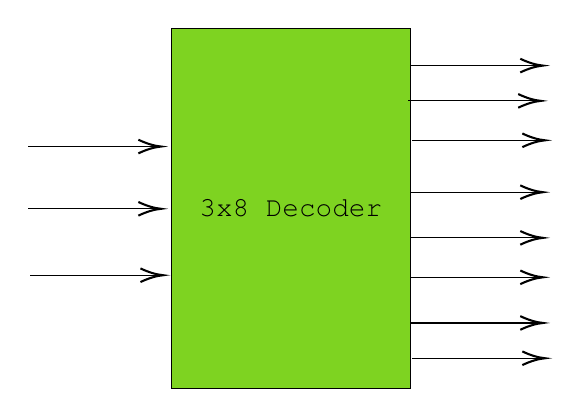
\begin{tikzpicture}[x=0.75pt,y=0.75pt,yscale=-1,xscale=1]
%uncomment if require: \path (0,300); %set diagram left start at 0, and has height of 300

%Shape: Rectangle [id:dp7384039086066188] 
\draw  [fill={rgb, 255:red, 126; green, 211; blue, 33 }  ,fill opacity=1 ] (282,44) -- (397,44) -- (397,217.5) -- (282,217.5) -- cycle ;
%Straight Lines [id:da2585166731802023] 
\draw    (213,101) -- (275,101) ;
\draw [shift={(277,101)}, rotate = 180] [color={rgb, 255:red, 0; green, 0; blue, 0 }  ][line width=0.75]    (10.93,-3.29) .. controls (6.95,-1.4) and (3.31,-0.3) .. (0,0) .. controls (3.31,0.3) and (6.95,1.4) .. (10.93,3.29)   ;
%Straight Lines [id:da7489396115344485] 
\draw    (213,131) -- (275,131) ;
\draw [shift={(277,131)}, rotate = 180] [color={rgb, 255:red, 0; green, 0; blue, 0 }  ][line width=0.75]    (10.93,-3.29) .. controls (6.95,-1.4) and (3.31,-0.3) .. (0,0) .. controls (3.31,0.3) and (6.95,1.4) .. (10.93,3.29)   ;
%Straight Lines [id:da33774516952405176] 
\draw    (214,163) -- (276,163) ;
\draw [shift={(278,163)}, rotate = 180] [color={rgb, 255:red, 0; green, 0; blue, 0 }  ][line width=0.75]    (10.93,-3.29) .. controls (6.95,-1.4) and (3.31,-0.3) .. (0,0) .. controls (3.31,0.3) and (6.95,1.4) .. (10.93,3.29)   ;
%Straight Lines [id:da21137181002513517] 
\draw    (396,79) -- (458,79) ;
\draw [shift={(460,79)}, rotate = 180] [color={rgb, 255:red, 0; green, 0; blue, 0 }  ][line width=0.75]    (10.93,-3.29) .. controls (6.95,-1.4) and (3.31,-0.3) .. (0,0) .. controls (3.31,0.3) and (6.95,1.4) .. (10.93,3.29)   ;
%Straight Lines [id:da6636989945396606] 
\draw    (398,98) -- (460,98) ;
\draw [shift={(462,98)}, rotate = 180] [color={rgb, 255:red, 0; green, 0; blue, 0 }  ][line width=0.75]    (10.93,-3.29) .. controls (6.95,-1.4) and (3.31,-0.3) .. (0,0) .. controls (3.31,0.3) and (6.95,1.4) .. (10.93,3.29)   ;
%Straight Lines [id:da30317065956331735] 
\draw    (397,123) -- (459,123) ;
\draw [shift={(461,123)}, rotate = 180] [color={rgb, 255:red, 0; green, 0; blue, 0 }  ][line width=0.75]    (10.93,-3.29) .. controls (6.95,-1.4) and (3.31,-0.3) .. (0,0) .. controls (3.31,0.3) and (6.95,1.4) .. (10.93,3.29)   ;
%Straight Lines [id:da4133576493028198] 
\draw    (397,145) -- (459,145) ;
\draw [shift={(461,145)}, rotate = 180] [color={rgb, 255:red, 0; green, 0; blue, 0 }  ][line width=0.75]    (10.93,-3.29) .. controls (6.95,-1.4) and (3.31,-0.3) .. (0,0) .. controls (3.31,0.3) and (6.95,1.4) .. (10.93,3.29)   ;
%Straight Lines [id:da6233332527453547] 
\draw    (397,164) -- (459,164) ;
\draw [shift={(461,164)}, rotate = 180] [color={rgb, 255:red, 0; green, 0; blue, 0 }  ][line width=0.75]    (10.93,-3.29) .. controls (6.95,-1.4) and (3.31,-0.3) .. (0,0) .. controls (3.31,0.3) and (6.95,1.4) .. (10.93,3.29)   ;
%Straight Lines [id:da7099313093237397] 
\draw    (397,186) -- (459,186) ;
\draw [shift={(461,186)}, rotate = 180] [color={rgb, 255:red, 0; green, 0; blue, 0 }  ][line width=0.75]    (10.93,-3.29) .. controls (6.95,-1.4) and (3.31,-0.3) .. (0,0) .. controls (3.31,0.3) and (6.95,1.4) .. (10.93,3.29)   ;
%Straight Lines [id:da42818070456886026] 
\draw    (398,203) -- (460,203) ;
\draw [shift={(462,203)}, rotate = 180] [color={rgb, 255:red, 0; green, 0; blue, 0 }  ][line width=0.75]    (10.93,-3.29) .. controls (6.95,-1.4) and (3.31,-0.3) .. (0,0) .. controls (3.31,0.3) and (6.95,1.4) .. (10.93,3.29)   ;
%Straight Lines [id:da5789580529374591] 
\draw    (397,62) -- (459,62) ;
\draw [shift={(461,62)}, rotate = 180] [color={rgb, 255:red, 0; green, 0; blue, 0 }  ][line width=0.75]    (10.93,-3.29) .. controls (6.95,-1.4) and (3.31,-0.3) .. (0,0) .. controls (3.31,0.3) and (6.95,1.4) .. (10.93,3.29)   ;

% Text Node
\draw (339.5,130.75) node   [align=left] {{\fontfamily{pcr}\selectfont 3x8 Decoder}};


\end{tikzpicture}

             \end{frame}
             
             
             \begin{frame}
             	\frametitle{ROM Example}
             	\centering
             	\includegraphics[width=0.8\textwidth]{ROM}
             \end{frame}
             
             \begin{frame}
             	\frametitle{ROM Example}
             	\centering
             	\includegraphics[width=0.8\textwidth]{rom-truthtable}
             \end{frame}
             
             \begin{frame}
             	\frametitle{Disadvantages of ROM}
             	\begin{itemize}
             		\item Real Life
             		\begin{itemize}
             			\item Can never be changed
             			\item Only realistic to manufacture in huge batches, and takes a lot of R\&D to get right
             			\item No software patches
             		\end{itemize}
             		\item Minecraft
             		\begin{itemize}
             			\item Can't be changed with outside influence (as easily)
             			\item In that sense, lines can never be repurposed without manual reconfiguration
             		\end{itemize}
             	\end{itemize}
             	
             \end{frame}
             
             \begin{frame}
             	\frametitle{Other types of ROM}
             	\begin{itemize}
             		\item \textbf{PROM}, \textbf{EPROM}, \textbf{EEPROM}
             		\item \textit{"Finally, a PROM that all computer science/engineering majors can enjoy" \newline -Aki, probably}
             		\item Essentially, these are just QOL improvements upon ROM
             		\item EPROM and EEPROM are the same in functionality, it's just that one is erased via ultraviolet light and  electrical signals
             	\end{itemize}
             \end{frame}
             
             \begin{frame}
             	\frametitle{PROM Advantages}
             	\begin{itemize}
             		\item PROMs are highly versatile, and it turns out that they are highly useful to implement minimum functions
             		\item e.g. $\lnot$ AB+AB can be minimized to B
             		\item We can explore this further using Karnaugh Maps
             		\begin{itemize}
             			\item Karnaugh Maps and minimization will be covered in an online video (this is a 1 credit class)
             		\end{itemize}
             	\end{itemize}
             \end{frame}
             
   		\begin{frame}
                \vfill
                \centering
                \begin{beamercolorbox}[sep=8pt,center,shadow=true,rounded=true]{title}
                    \usebeamerfont{title}Grading / Open OH / Project 5\par%
                \end{beamercolorbox}
                \vfill
             \end{frame}
   		
    
\end{document}
